\documentclass[12pt]{article}

\usepackage[utf8x]{inputenc} % Включаем поддержку UTF8  
\usepackage[russian]{babel}  % Включаем пакет для поддержки русского языка  
\usepackage{hyperref}        % Для гиперссылок

% Математика
\usepackage{amsmath}         % В т.ч. для матриц
\usepackage{amssymb}

% Прога
\usepackage{etoolbox}
\usepackage{listings}

% Цвета
\usepackage{xcolor}

% Картинки
\usepackage{graphicx}
\graphicspath{ {./images/} }

\newtheorem{property}{Свойство}
\newtheorem{consequence}{Следствие}[property]

\newcommand{\qedsymbol}{\rule{2mm}{2mm}}

\begin{document}

\thispagestyle{empty}
\begin{center}
\textbf{ПРАВИТЕЛЬСТВО РОССИЙСКОЙ ФЕДЕРАЦИИ}

\vspace{5ex}
	
\textbf{Федеральное государственное автономное образовательное учреждение \\ высшего образования \\ <<Национальный исследовательский университет \\ <<Высшая школа экономики>>}
\end{center}
\vspace{5ex}

\begin{center}
    Московский институт электроники и математики им. А.Н. Тихонова  
    
    \vspace{5ex}
    
    Департамент прикладной математики
    
    \vspace{10ex}
    \textbf{Отчёт \\ по лабораторной работе №7 \\ по курсу <<Алгоритмизация и программирование>>}
	\vspace{7ex}

\end{center}

\begin{center} 
\begin{tabular}{| p{0.3\linewidth}| p{0.3\linewidth}| p{0.3\linewidth}|}
 \hline	
ФИО студента & Номер группы & Дата \\  \hline
 & & \\  
Вязов Глеб \newline Дмитриевич & БПМ-231 & 17.01.2024\\  
 & & \\  \hline		
\end{tabular}
\end{center}

\begin{center}
	\vspace{3ex}
	
	\vfill
   
   \normalsize
    
	\textbf{Москва, 2023}
\end{center}

\newpage

%---------------------------------------------------------------------------------

\section*{Задание (вариант №7)}
Написать функцию обработки строки и программу, тестирующую данную функцию. В программе должен быть предусмотрен вывод исходной строки, которая при выделении слов не должна измениться.

Дана строка, содержащая от 1 до 30 слов, в каждом из которых от 1 до 10 латинских букв и/или цифр; между соседними словами – не менее одного пробела, за последним словом – точка. Напечатать все слова, отличные от последнего слова, предварительно преобразовав каждое из них по следующему правилу: оставить в слове только первые вхождения каждой буквы.

\newpage

%---------------------------------------------------------------------------------

\section*{Решение}\addcontentsline{toc}{section}{Решение}

\lstset{ %
texcl=true,%
language=C,                 % выбор языка для подсветки
basicstyle=\small\sffamily, % размер и начертание шрифта для подсветки кода
numbers=left,               % где поставить нумерацию строк (слева\справа)
numberstyle=\tiny,           % размер шрифта для номеров строк
stepnumber=1,                   % размер шага между двумя номерами строк
numbersep=5pt,                % как далеко отстоят номера строк от подсвечиваемого кода
backgroundcolor=\color{white}, % цвет фона подсветки - используем \usepackage{color}
showspaces=false,            % показывать или нет пробелы специальными отступами
showstringspaces=false,      % показывать или нет пробелы в строках
showtabs=false,             % показывать или нет табуляцию в строках
frame=single,              % рисовать рамку вокруг кода
tabsize=3,                 % размер табуляции по умолчанию равен 2 пробелам
captionpos=t,              % позиция заголовка вверху [t] или внизу [b] 
breaklines=true,           % автоматически переносить строки (да\нет)
breakatwhitespace=false, % переносить строки только если есть пробел
escapeinside={\%*}{*)},   % если нужно добавить комментарии в коде
inputencoding=utf8x,
extendedchars=\true
}

\begin{lstlisting}[label=string_code1,caption=C]
#include <stdio.h>
#include <stdlib.h>
#include <string.h>
#include <windows.h>

#define LEN 300

char* get_unique_char(char* word, int len) {
    int i, k = 0;
    for (i=0; i<len; i++) {
        // Поиск первого вхождения буквы word[i] в слово word.
        // Возвращает указатель на первое вхождение символа в строке
        // Сравниваем указателем на текущую букву
        if (strchr(word, word[i]) != &word[i]) {
            k++;
        } else {
            word[i-k] = word[i];
        }
    }
    word[i-k] = '\0';
    word = realloc(word, (i-k) * sizeof(char));
    return word;
}

// Фукнция создает строку (массив символов) на основе string
// Значения: string[firstindex], ..., string[lastindex-1]
// Длина слова: lastindex - firstindex
char* create_string(char string[], int first_index, int last_index) {
    char *word = calloc(last_index - first_index, sizeof(char));
    for (int i=first_index; i<last_index; i++) {
        word[i-first_index] = string[i];
    }
    return word;
}

// Функция возвращает последнее слово -- указатель на массив символов
char* get_last_word(char string[], int* len_string) {
    int index = 0;
    int first_index = 0;

    // Находим длину строки - 1 (index) и индекс, с которого начинается последнее слово (firstindex)
    while (string[index] != '.') {
        if (string[index] == ' ') {
            first_index = index + 1;
        }
        index++;
    }

    // Сохраняю длину массива (не учитывая точку) и создаю массив символов -- последнее слово
    *len_string = index;
    return create_string(string, first_index, index);
}

void task(char string[], char* last_word, int len_string) {
    /* 1. Переменная first_index отвечает за первый индекс в слове. Прохожусь циклом по исходной строке.
     * 2. Если наткнулся на пробел, то создаю слово word: string[first_index], ..., string[i-1]
     * 3. Сравниваю с последним. Если равны (то есть strcmp = 0), то пропускаю его
     * 4. Вывожу только первые вхождения каждой буквы с помощью функции print_unique_char()
     */
    int first_index = 0;

    for (int i=0; i<len_string+1; i++) {
        if (string[i] == ' ') {
            // Обработка случая нескольких пробелов подрят
            if (string[first_index] == ' ') {
                first_index = i + 1;
                printf(" ");
                continue;
            }

            char* word = create_string(string, first_index, i);
            if (strcmp(last_word, word) == 0) { // Слова равны
                first_index = i + 1;
                continue;
            }

            char* unique_string = get_unique_char(word, i-first_index);
            printf(" %s", unique_string);

            first_index = i + 1;

            free(unique_string);
        }
    }
    printf(".");
}

int main() {
    // Меняем кодировку на UTF-8, чтобы можно было писать на русском
    SetConsoleOutputCP(CP_UTF8);
    // Ввод переменных. Дружественный интерфейс
    printf("Выполнил задание: Вязов Глеб. Группа: БПМ231\n");

    char string[LEN];
    int len_string;

    // Считываем строку из стандартного потока stdin
    gets(string);
    printf("Введённая строка: %s", string);

    char *last_word = get_last_word(string, &len_string);
    printf("\nПоследнее слово: %s", last_word);
    printf("\nОтвет:");
    task(string, last_word, len_string);

    printf("\nИзначальная строка (неизмененная): %s", string);

    free(last_word);

    return 0;
}
\end{lstlisting} 

\newpage

%---------------------------------------------------------------------------------

\section*{Тестирование}

\begin{enumerate}

\item \textbf{Тест №1.}

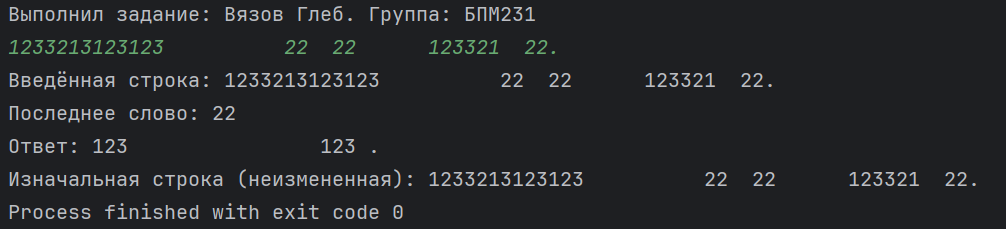
\includegraphics[width=1\textwidth]{img1}



\item \textbf{Тест №2.}

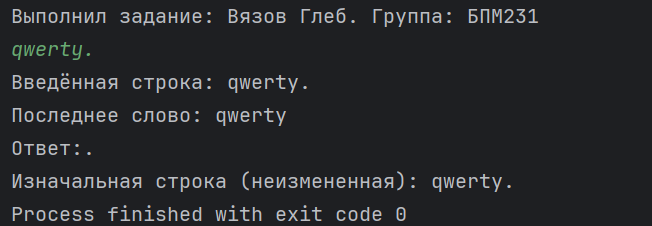
\includegraphics[width=1\textwidth]{img2}



\item \textbf{Тест №3.}

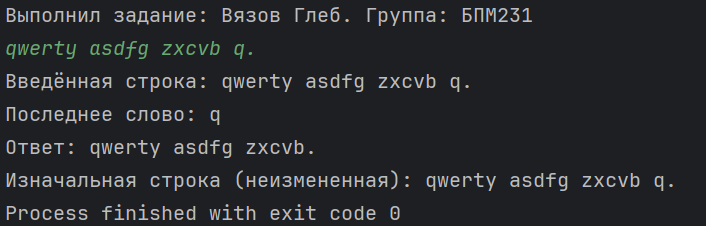
\includegraphics[width=1\textwidth]{img3}


\end{enumerate}


\end{document}
